%% TODO
% [] Clear the TRACKING CHANGES comments in this document.
% [] BIBTEX currently causes 5 errors whenever we cite anything.
% [] Improve on the dark theme, I currently just used a quick and dirty trick. For alternatives: https://tex.stackexchange.com/questions/57477/beamer-dark-theme
% [✓] Add wikimedia HR for comparison
% [✓] Use the PROJECT PLAN to write the 'What are we using MESA' for section.
% [✓] Add captions to what does it look like.
% [] Briefly go over INLISTS.
% [] Write about the fact that mass is transfered via the ROCHE LOBE via the Lagrangian point and not via the 
% Add overleaf to the GIT repo.
% [] Consider the addition of subsections in the TOC. 
% [] Consider frame subtitles.
% [] Check the TENSES of the texts on the slides.
% [] Contemplate interesting results we can takeaway from the results.
% [] Write the results.
% [] Write the takeaway / conclusion / discussion.
% [] Add the reference slide.
%
%% REFERENCE MATERIAL
% Quick tutorial on creating SLIDES in latex: https://www.overleaf.com/learn/latex/Beamer

\documentclass{beamer}
\usepackage[utf8]{inputenc}
\usepackage{amsmath}
\usepackage{amssymb}
\usepackage{bm}
\usepackage{physics}
\usepackage{siunitx}
\usepackage{hyperref}
\usepackage{graphicx}
\usepackage[numbers]{natbib} % https://www.bibtex.com/
\usepackage{media9} % For animations

% Dark theme
\setbeamercolor{frametitle}{fg=white}
\setbeamercolor{background canvas}{bg=black}
\setbeamercolor{normal text}{fg=white}

%\usetheme{CambridgeUS}

% For media9
\graphicspath{./figs}
\addmediapath{./movs}

% Figure numbering
\setbeamertemplate{caption}[numbered]

% Have numbering in the TOC.
\setbeamertemplate{section in toc}[sections numbered]
\setbeamertemplate{subsection in toc}[subsections numbered]

\title{Simulating binary star systems with MESA}
\author{Rembrand Ruppert \and Iris Draijer \and Kaydo Alders}
\institute[UvA] % (optional)
{
  University of Amsterdam\\
  Anton Pannekoek institute\\
  Supervisor: Philipp Moestra
}
\date[\today]{\today}
\logo{
\includegraphics[height=0.5cm]{figs/uva_logo.png}}
\date{Project symposium, Februari 2022}

\begin{document}

\frame{\titlepage}

\begin{frame}{Outline}
    \tableofcontents
\end{frame}

\section{Introduction to MESA and our small project}
%% Script
% Modules for Experiments in Stellar Astrophysics (MESA) is an open source code library and simulation program for the simulation of stellar objects in one-dimension. MESA is used to calculate evolution tracks of stellar objects and to determine at any time properties such as the mass, metallicity, temperature, density, angular momentum, age of the stellar object, nuclear rates, atmosphere, types of heat transfer  at different stages of its lifetime. 

%\subsection{MESA in short}
\begin{frame}{What is MESA?}
    \begin{itemize}
        \item<1-> \textit{MESA} stands for \textit{Modules for Experiments in Stellar Astrophysics}.
        \item<2-> It is a code library that is used to simulate stellar objects throughout their lifetimes. %\cite{Paxton2011, Paxton2013, Paxton2015, Paxton2018, Paxton2019, Jermyn2022}.
    \end{itemize}
\end{frame}

%% Script
% In this project, we will use MESA to investigate the effects of MASS TRANSFER between two stars in binary systems. We compare the properties of the accretor after a transfer of mass from the donor to the properties of the same stellar objects as they are found in isolation.
%
% - Say aloud HR as Hertzsprung Russel and give a short explanation and give refer to the upcoming slides. 
% - Motivate why we are interested in what we are interested in.
%\subsection{What we do and motivation for the project}
\begin{frame}{What are we using MESA for?}
    \begin{itemize}
        \item<1-> We will use MESA to simulate \alert{binary star systems} and consider the \alert{mass transfer} between them.
        \item<2-> We then compare the resulting stars with their isolated counterparts.
        \item<3-> In particular, we are interested  in 
        \begin{enumerate}
            \item<4-> Comparing the \alert{HR-diagrams} and \alert{ $T$-$\rho$ profiles} of the stars in the binary system to the isolated stars.
            \item<5-> Obtaining information on the binary system, such as the \alert{mass transfer rate} and \alert{state variables} of the individual stars.
        \end{enumerate}
    \end{itemize}
\end{frame}

%% Script
% The comparison of these properties provides valuable information on the differences between stars in binary systems and stars in isolation.
% - The STATISTIC on binary systems from Iris' project plan.
% - ALGOL PARADOX: A situation that can occur in binaries, for instance, is that a star of lesser mass is more advanced in its evolution than its companion of greater mass. This is not observed when we compare the stars in isolation. A fortiori, the equations that determine stellar evolution dictate that a star of lesser mass always evolves less rapidly than a star of greater mass.  
\begin{frame}{Why consider binary systems?}
    \begin{itemize}
        \item<1-> \alert{$X\%$} of stars are not in isolated systems but in binaries instead.
        \item<2-> Binaries produce interesting configurations, such as that of the famous \alert{Algol paradox}.
    \end{itemize}
\end{frame}

% 1Msun, 02Z star DEMO
\begin{frame}{What does it look like?}
    \begin{columns}
        \begin{column}{0.5\textwidth}
            \begin{center}
                \begin{figure}
                    % Note: These include media that start here and will follow are animations; only some pdf readers will ne able to play them.
                    \includemedia[activate=pagevisible, width=\textwidth ]{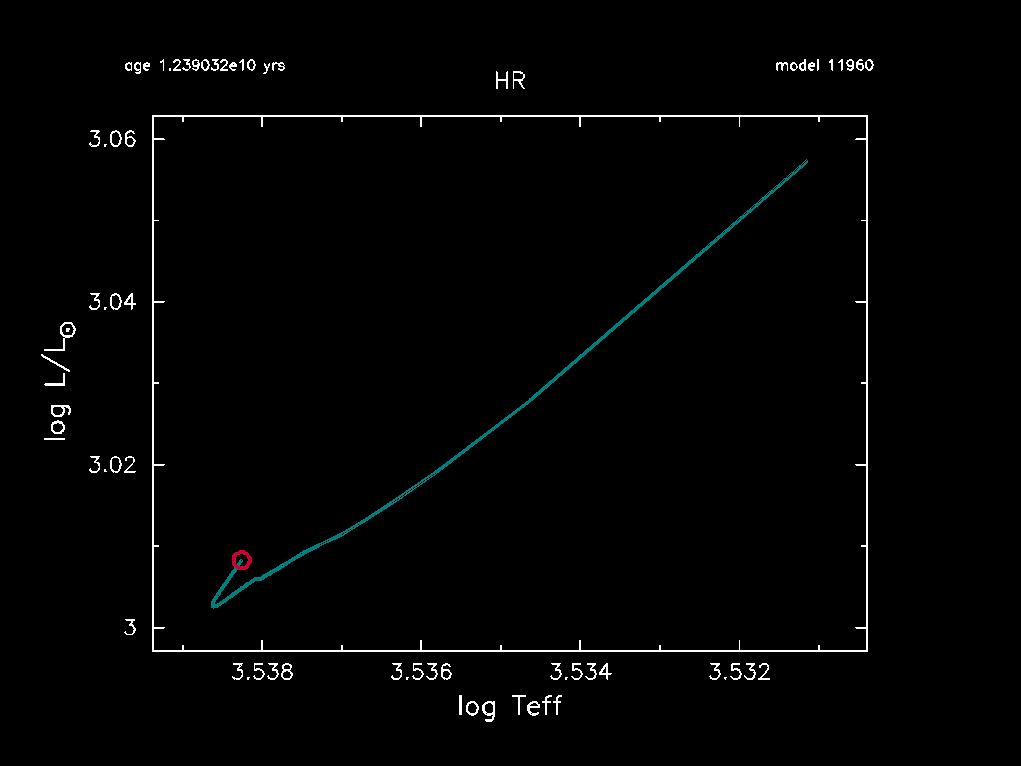
\includegraphics{figs/hr_test.png}}{hr/hr_1M_02Z.mp4}
                    \caption{Simulated evolutionary track of a $1 M_\odot$, $0.2Z$ star.}
                    \label{fig:hr_1M_02Z}
                    \end{figure}
            \end{center}
        \end{column}
        \begin{column}{0.5\textwidth}
            \begin{center}
                \begin{figure}
                    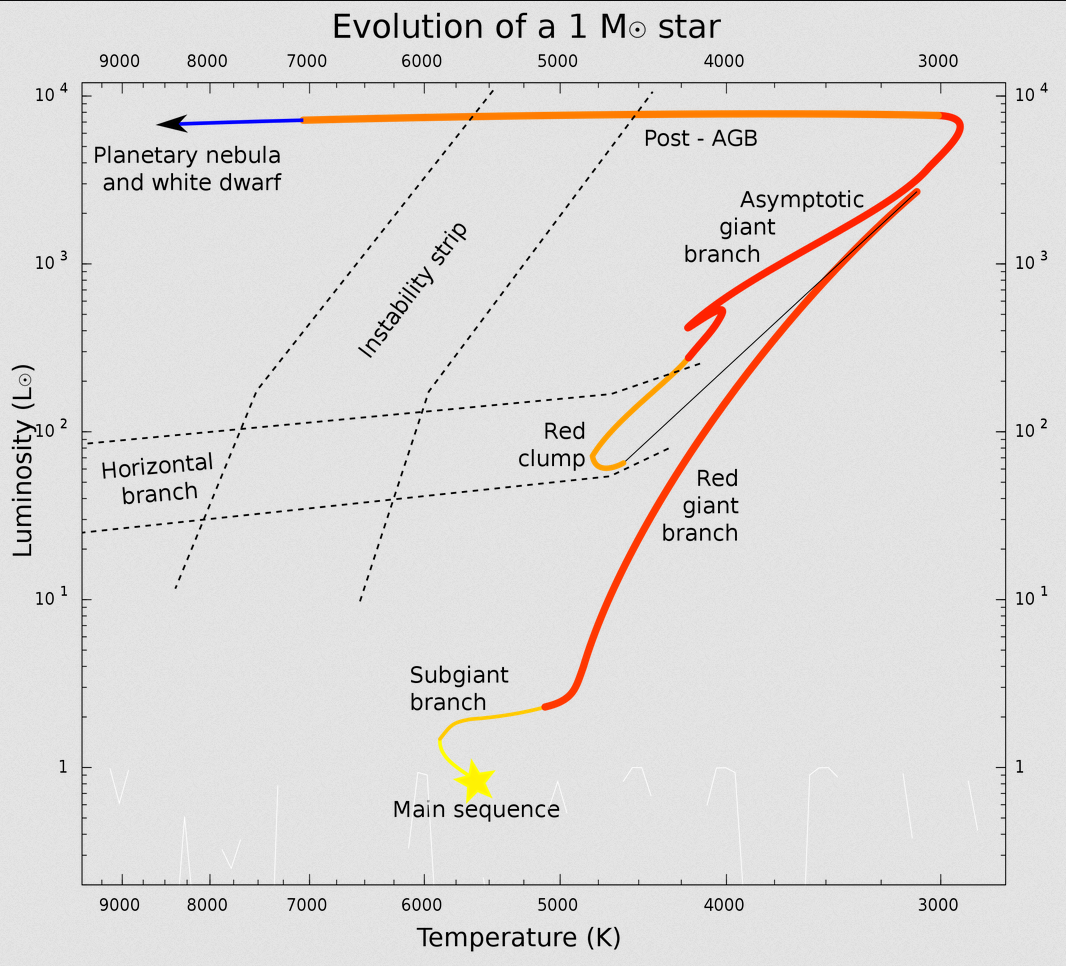
\includegraphics[width=\textwidth]{figs/hr_example_1m}
                    \caption{Example Evolutionary track of a $1 M_\odot$ star. src: Wikimedia Commons, Lithopsian}
                    \label{fig:hr_example_1m}
                \end{figure}
            \end{center}
        \end{column}
    \end{columns}      
\end{frame}

%% Script
% - Show case of what we can do in MESA, these are not yet our final results but from the explorative phase of figuring out what we can do with MESA. 
\begin{frame}{What does it look like?}
    \begin{center}
        \begin{figure}
            \includemedia[activate=pagevisible, width=0.8\textwidth ]{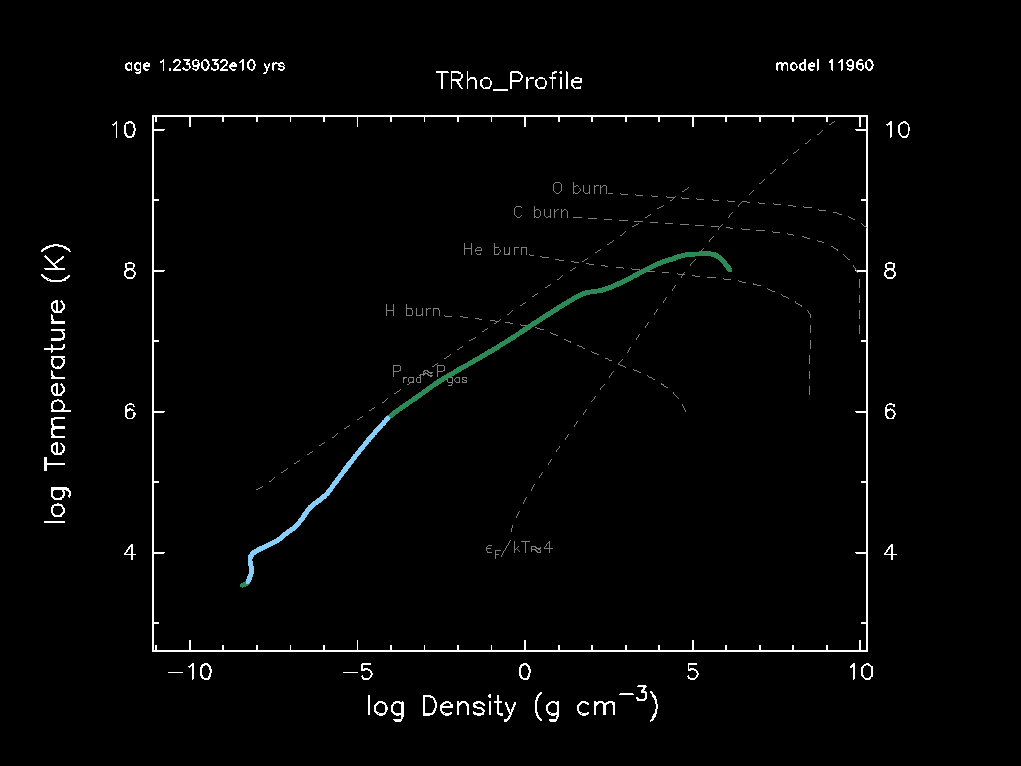
\includegraphics{figs/trho_test.png}}{trho/trho_profile_1M_02Z.mp4}
            \caption{Temperature - density profile of a simulated $1M_\odot$ star throughout its lifetime.}
            \label{fig:trho_1M_02Z}
        \end{figure}
    \end{center}
\end{frame}

% 10Msun, 04Z star DEMO
\begin{frame}{What does it look like?}
    \begin{columns}
        \begin{column}{0.5\textwidth}
            \begin{center}
                \begin{figure}
                    \includemedia[activate=pagevisible, width=\textwidth ]{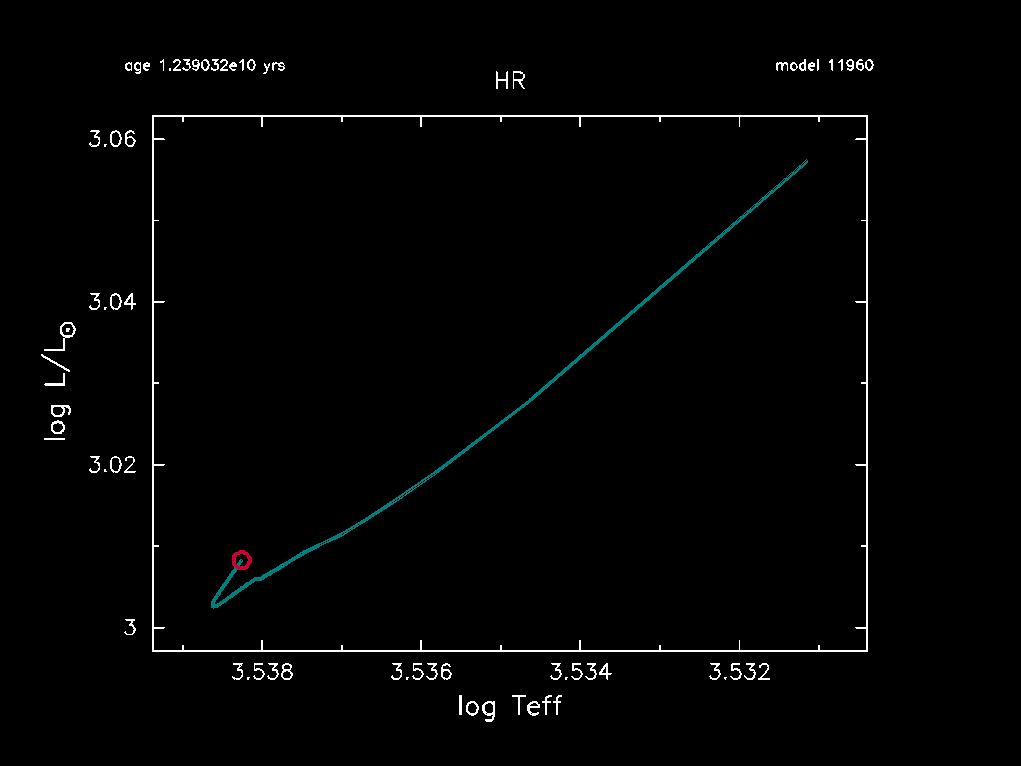
\includegraphics{figs/hr_test.png}}{hr/hr_10M_04Z.mp4}
                    \caption{Hertzsprung-Russel diagram of $10M_\odot$, $0.4Z$ star}
                \end{figure}
            \end{center}
        \end{column}
        \begin{column}{0.5\textwidth}
            \begin{center}
                \begin{figure}
                    \includemedia[activate=pagevisible, width=\textwidth ]{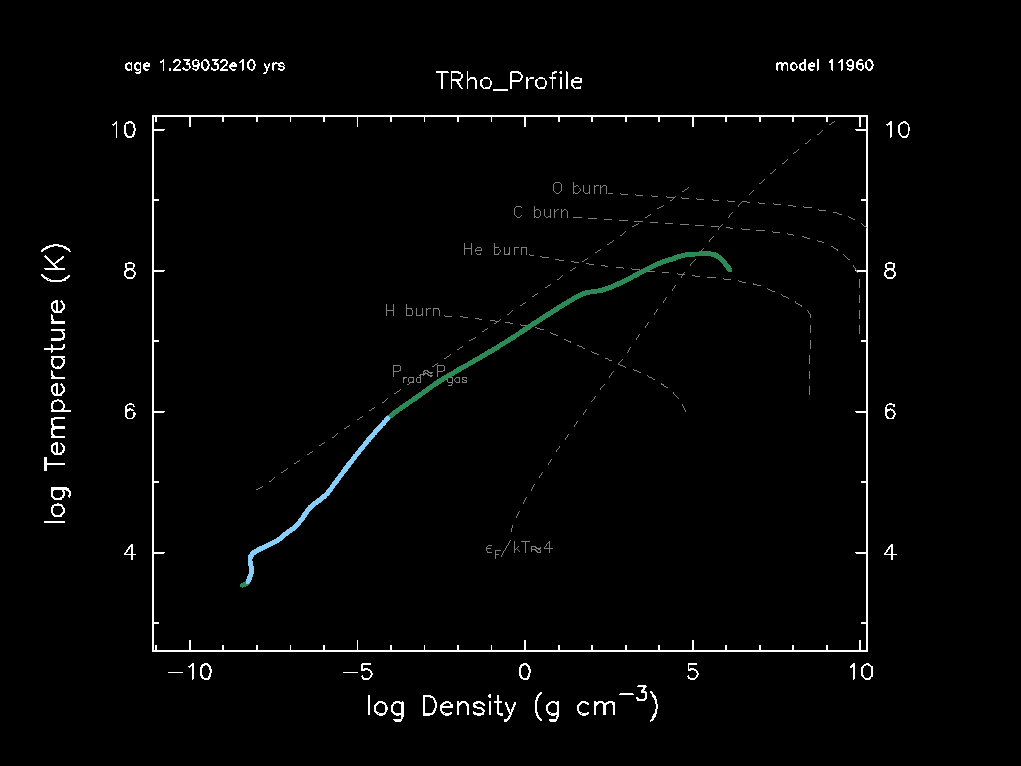
\includegraphics{figs/trho_test.png}}{trho/trho_profile_10M_04Z.mp4}
                    \caption{Temperature density profile of a $10M_\odot$, $0.4Z$ star}
                \end{figure}
            \end{center}
        \end{column}
    \end{columns}      
\end{frame}

% Optional 50Msun, 02Z star DEMO
\begin{frame}{What does it look like?}
    \begin{columns}
        \begin{column}{0.5\textwidth}
            \begin{center}
                \begin{figure}
                    \includemedia[activate=pagevisible, width=\textwidth ]{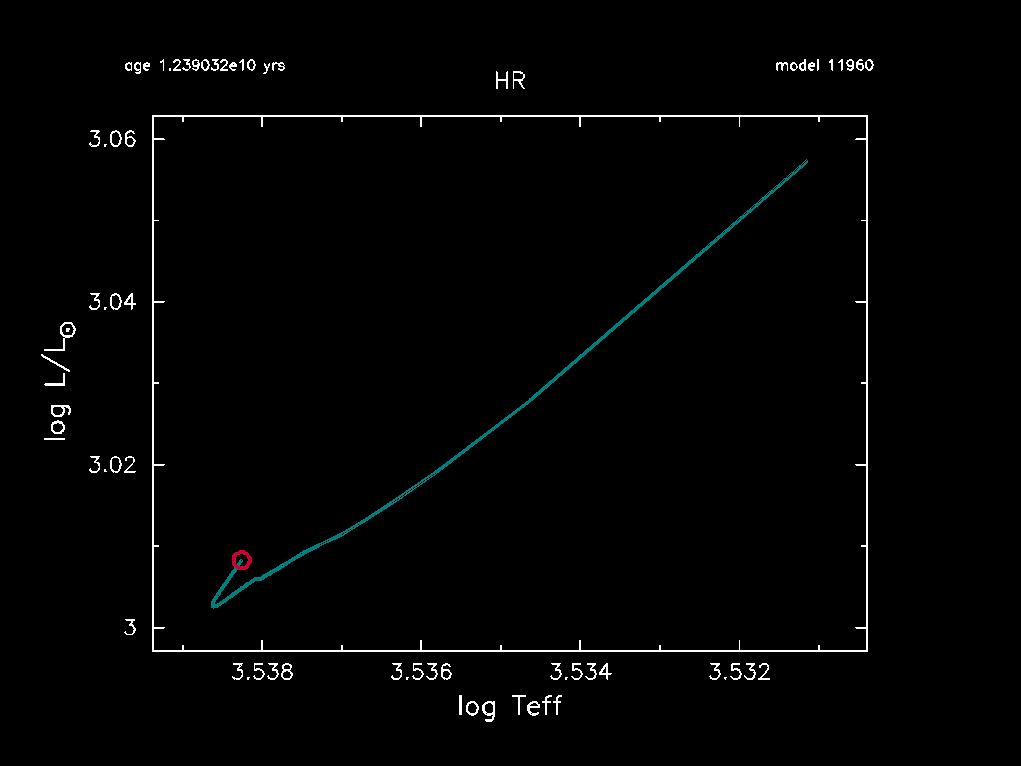
\includegraphics{figs/hr_test.png}}{hr/hr_50M_02Z.mp4}
                    \caption{Hertzsprung-Russel diagram of a $50M_\odot$, $0.2Z$ star}
                \end{figure}
            \end{center}
        \end{column}
        \begin{column}{0.5\textwidth}
            \begin{center}
                \begin{figure}
                    \includemedia[activate=pagevisible, width=\textwidth ]{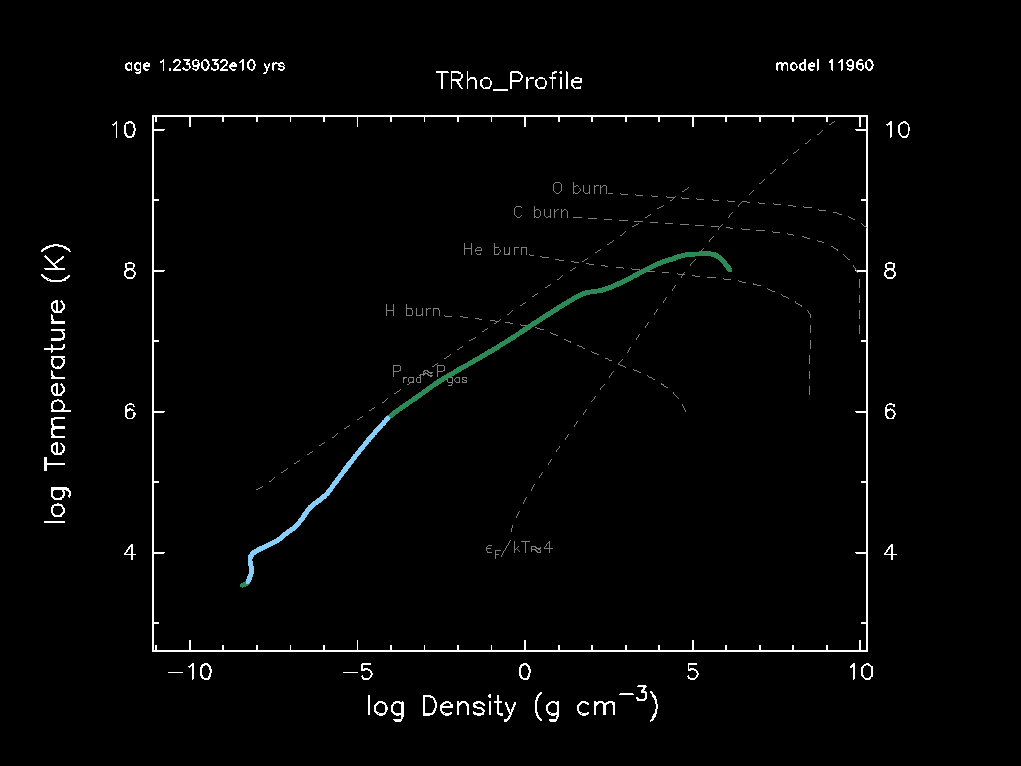
\includegraphics{figs/trho_test.png}}{trho/trho_profile_50M_02Z.mp4}
                    \caption{Temperature density profile of $50M_\odot$, $0.2Z$ star}
                \end{figure}
            \end{center}
        \end{column}
    \end{columns}      
\end{frame}

% Binary star system DEMO
\begin{frame}{What does it look like?}
    \begin{center}
        \begin{figure}
            \includemedia[activate=pagevisible, width=\textwidth ]{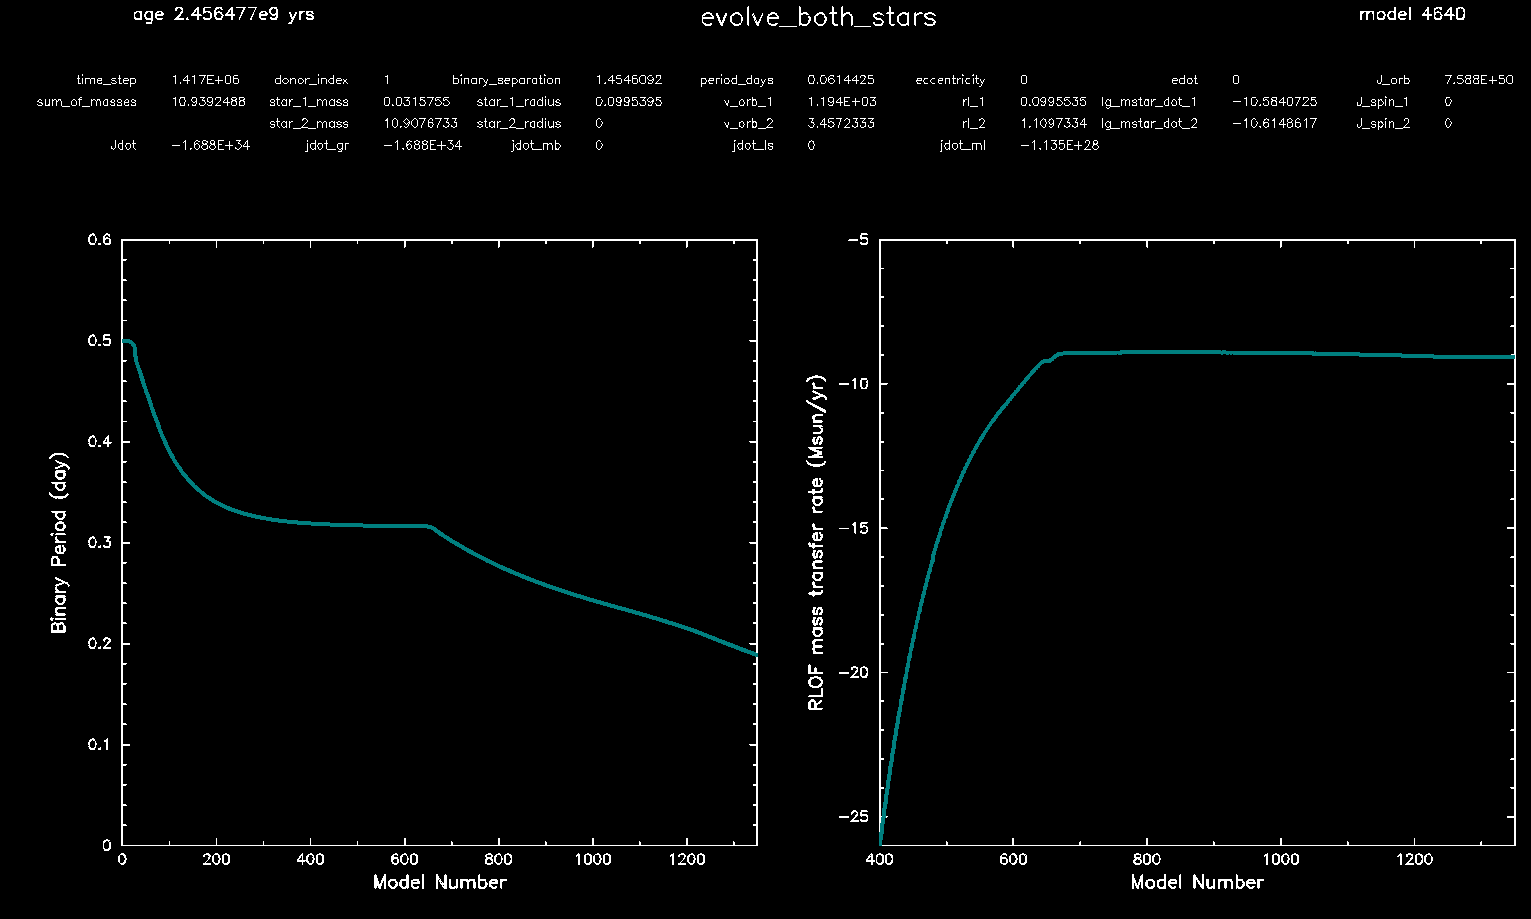
\includegraphics{figs/grid_test.png}}{grid/grid1.mp4}
            \caption{Binary system with increasingly smaller orbital period. Left: orbital period against model number. Right: Mass transfer rate against model number.}
        \end{figure}
    \end{center}
\end{frame}

% Double black hole test suite DEMO.
% - This is just here to show the many other things that MESA offers.
\begin{frame}{What does it look like?}
    \begin{center}
        \begin{figure}
            \centering
            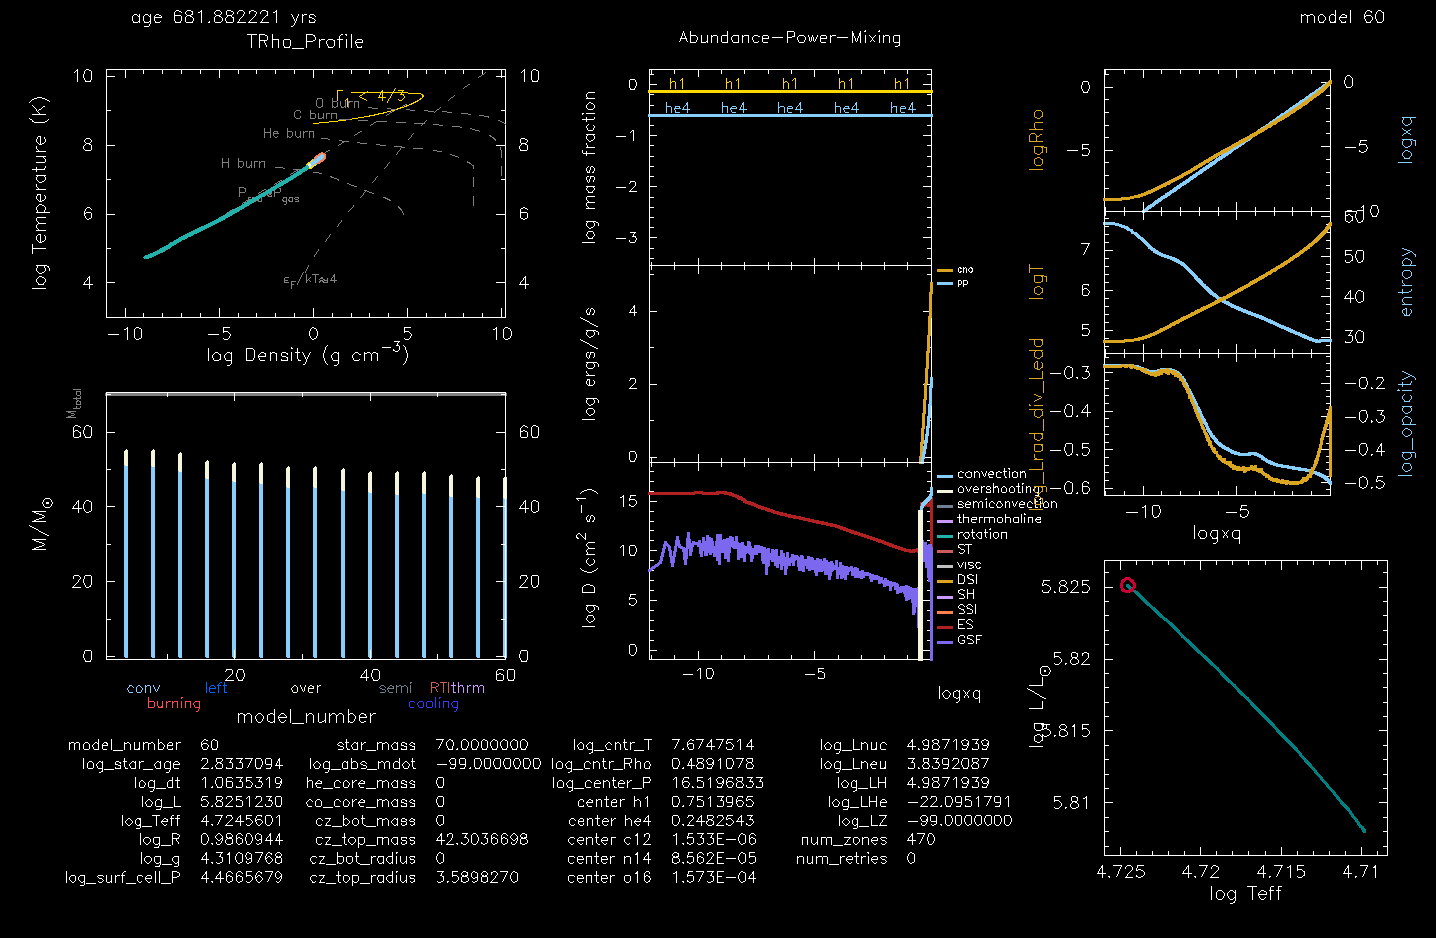
\includegraphics[width=\textwidth]{figs/double_bh}
            \caption{Test run with two stars that become black holes.}
            \label{fig:double_bh_test}
        \end{figure}
    \end{center}
\end{frame}

\section{Configuring MESA for our project}
\begin{frame}{Configuring MESA}
    \framesubtitle{Structure of the library}
    \begin{columns}
        \begin{column}{0.5\textwidth}
            \begin{itemize}
                \item<1-> The library is written in Fortran and requires some basic knowledge of the language.
                \item<2-> The file in Fig.~\ref{fig:star_data_def} contains some declarations and subroutines that initialize the model of the star.
            \end{itemize}
        \end{column}
        \begin{column}{0.5\textwidth}
            \begin{center}
                \pause
                \begin{figure}
                    \centering
                    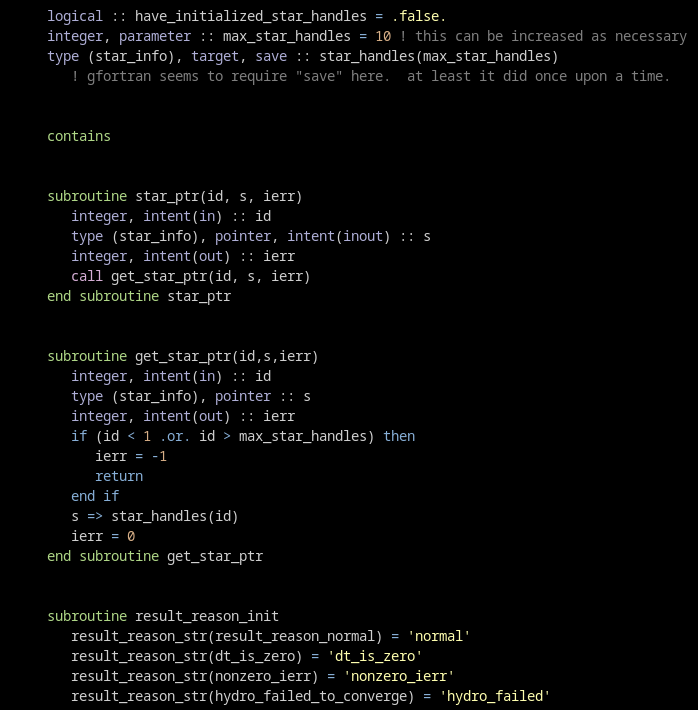
\includegraphics[width=\textwidth]{figs/star_data_def.png}
                    \caption{star\_data/public/star\_data\_def.f90}
                    \label{fig:star_data_def}
                \end{figure}
            \end{center}
        \end{column}
    \end{columns}      
\end{frame}

% This, together with the slides on the configuration files, is essentially the methods section of a paper.
\subsection{Mass transfer in binaries}
\begin{frame}{Mass transfer in binaries}
    \begin{itemize}
        \item<1-> There are two ways through which mass transfer can happen between two stars in a binary system. These are
        \begin{enumerate}
            \item<2-> Mass transfer through stellar winds.
            \item<3-> Mass transfer through \alert{Roche lobe overflow (RLOF)}.
        \end{enumerate}
        \item<4-> When considering the Roche lobe in a binary system, there are generally three possible cases
        \begin{enumerate}
            \item<5-> Detached binaries
            \item<6-> \alert{Semi-detached binaries}
            \item<7-> Contact binaries
        \end{enumerate}
        \item<8-> We consider mass transfer through RLOF with a semi-detached binary.
        \item<9-> The transfer of mass happens through the Lagrange point L1 (visualized on the next slide).
    \end{itemize}
\end{frame}

\begin{frame}{Mass transfer in binaries}
    \begin{figure}
        \begin{minipage}{0.7\textwidth}
            \centering
            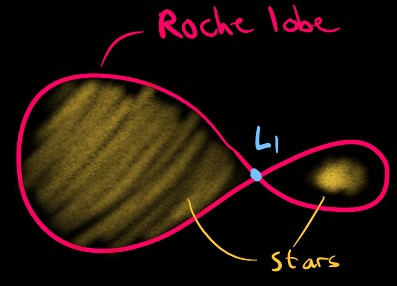
\includegraphics[width=0.5\textwidth]{figs/semi-detached_binary.jpg}
            \caption{Semi-detached binary}
            \label{fig:semi-detached_binary}        
        \end{minipage}
        \begin{minipage}{0.5\textwidth}
            \centering
            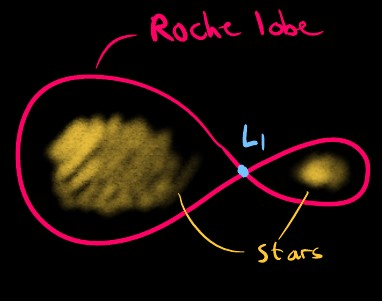
\includegraphics[width=0.5\textwidth]{figs/detached_binary.jpg}
            \caption{Detached binary}
            \label{fig:detached_binary}
        \end{minipage}%
        \begin{minipage}{0.5\textwidth}
            \centering
            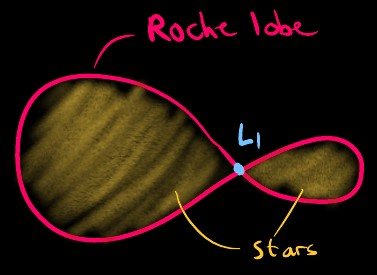
\includegraphics[width=0.5\textwidth]{figs/contact_binary.jpg}
            \caption{Contact binary}
            \label{fig:contact_binary}
        \end{minipage}
    \end{figure}
\end{frame}

\subsection{Setting up the configuration files}
\begin{frame}{Configuring MESA}
    \framesubtitle{Inlists}
    \begin{columns}
        \begin{column}{0.5\textwidth}
            \begin{itemize}
                \item<1-> MESA uses \alert{inlists}, which are Fortran files that are loaded on a run and which specify the configuration and other (many!) parameters of the simulation process.
                \item<2-> Fig.~\ref{fig:inlist_project_binary} specifies a subset of settings for the binary system.
                \item<3-> Individual settings for the stars, besides the initial mass and initial metallicity, are specified in separate inlists (not shown).
            \end{itemize}
        \end{column}
        \begin{column}{0.5\textwidth}
            \pause[2]
            \begin{figure}
                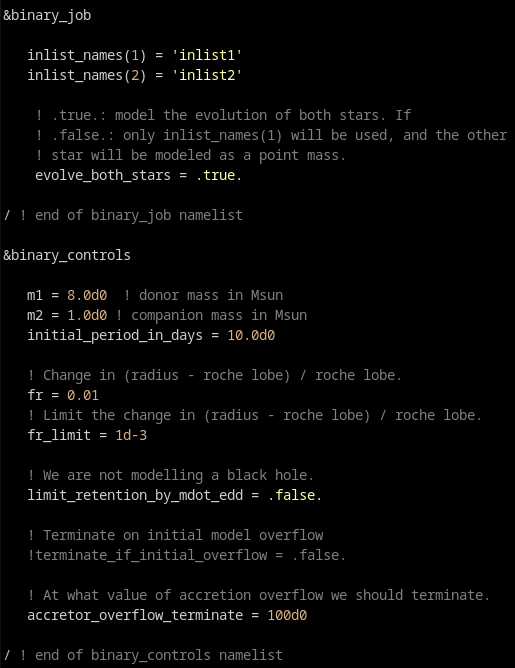
\includegraphics[width=0.9\textwidth]{figs/inlist_project_binary.png}
                \caption{Inlist that specifies some settings of the binary system.}
                \label{fig:inlist_project_binary}
            \end{figure}
        \end{column}
    \end{columns}
\end{frame}

\subsection{Setup for the simulations}
\begin{frame}{Setup for the simulations}
    \begin{itemize}
        \item<1-> We consider \alert{continuous mass transfer} through semi-detached RFOL that starts once the star enters the main sequence.
        \item<2-> We run simulations with respectively a $1M_\odot$, $2M_\odot$, $4M_\odot$ and $8M_\odot$ star as the \alert{accretor}, and a $5M_\odot$ as the \alert{donor} in the all cases.
        \item<3-> We then run simulations of \alert{isolated} $1M_\odot$, $2M_\odot$, $4M_\odot$ and $8M_\odot$ stars respectively.
        \item<4-> We consider the mass transfer rate in the binaries and compare the HR-diagrams and $T\rho$-profiles of the accretor with that of the isolated stars.
    \end{itemize}
\end{frame}

\section{Simulation outcomes}
\begin{frame}{Simulation outcomes}
\framesubtitle{$1M_\odot$ accretor}
\end{frame}
\begin{frame}{Simulation outcomes}
\framesubtitle{$2M_\odot$ accretor}
\end{frame}
\begin{frame}{Simulation outcomes}
\framesubtitle{$4M_\odot$ accretor}
\end{frame}
\begin{frame}{Simulation outcomes}
\framesubtitle{$8M_\odot$ accretor}
\end{frame}

\begin{frame}{Takeaways}
    \begin{itemize}
        \item Continuous mass transfer between the stars in the binaries results in vastly different and HR-diagrams that are unrecognizable from the theory for the isolated case.
        \item $\dots$
    \end{itemize}
\end{frame}

\section{Further research}
\begin{frame}{Further research}
     \begin{itemize}
         \item<1-> The possibilities with binary systems are endless! Some direction to go into with further research are
         
         \begin{enumerate}
             \item<2-> A consideration changes in heat transfer mechanisms (i.e. convection and radiation) upon mass transfer.
             \item<3-> A consideration contact binaries. 
             \item<4-> A consideration non-continuous mass transfer, i.e. RLOF that starts and ends at a particular age of the star or under particular A constitutiveation conditions of the star.
             \item<5-> A consideration stellar wind mass transfer.
             \item<6-> A consideration other types of stellar objects such as red / blue / black dwarfs, neutron stars and black holes.
             \item<7-> Finally, the particularly ambitious research project can consider simulating trinary systems or even $N$-stars systems.
             \end{enumerate}
     \end{itemize}
\end{frame}

\begin{frame}
    %\nocite{Paxton2011, Paxton2013, Paxton2015, Paxton2018, Paxton2019, Jermyn2022}
    \bibliographystyle{science}
    \bibliography{bib.bib}
\end{frame}

\end{document}